% Appendix Template

\chapter{Pico Grammar} % Main appendix title

\label{app:pico} % Change X to a consecutive letter; for referencing this appendix elsewhere, use \ref{AppendixX}

\section{Original definition} \label{app:pico:default}
\lstinputlisting[language=RascalGrammar, caption={The Pico language as a Rascal grammar}]{Code/grammars/pico/Pico.grammar}

\subsection{Simplified without priority} \label{app:picosimple}
\lstinputlisting[language=RascalGrammar, caption={The plain grammar with priority removal}]{Code/grammars/pico/plain.grammar}

\subsection{Strongly Regular} \label{app:pico:stronglyregular}
\lstinputlisting[language=RascalGrammar, caption={The strongly regular approximation of the original grammar}]{Code/grammars/pico/stronglyregular.grammar}


\pagebreak\subsection{NFA for strongly regular WhitespaceAndComment}
\begin{figure}[h!]
	\centering
	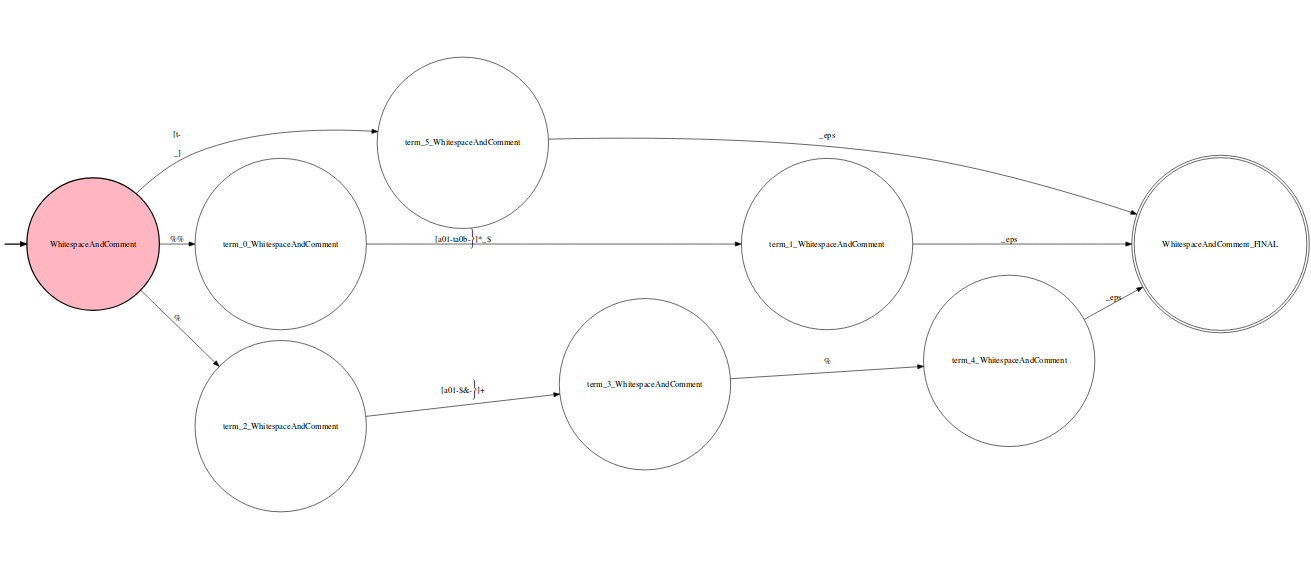
\includegraphics[width=\textwidth, keepaspectratio]{Figures/pico_nfa_whitespaceandcomment.png}
	\decoRule
 	\caption[NFA of WhitespaceAndComment]{The NFA for WhitespaceAndComment, produced from the strongly regular approximation. Used in the prototype context. The weird characterclasses are equal to ![\%] and ![$\backslash$ n]}
 	\label{fig:pico:NFA:WhitespaceAndComment}
\end{figure}


\subsection{DFA for strongly regular WhitespaceAndComment}
\begin{figure}[h!]
	\centering
	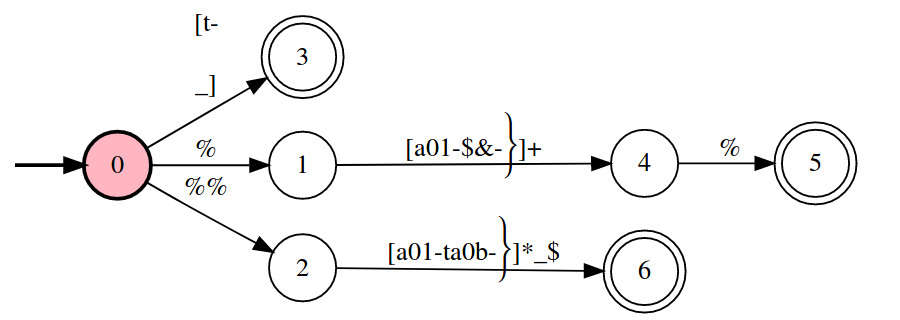
\includegraphics[width=\textwidth, keepaspectratio]{Figures/pico_dfa_whitespaceandcomment.png}
	\decoRule
 	\caption[DFA of WhitespaceAndComment]{The DFA for WhitespaceAndComment, produced from the strongly regular approximation. Used in the prototype context. The weird characterclasses are equal to ![\%] and ![$\backslash$ n]}
 	\label{fig:pico:DFA:WhitespaceAndComment}
\end{figure}


\pagebreak\subsection{Results of generated highlighter}
\begin{figure}[h]
	\centering
	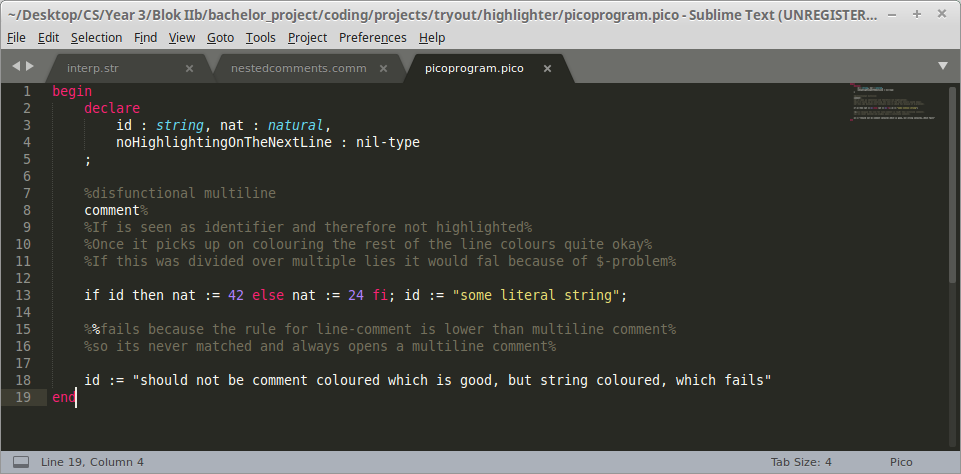
\includegraphics[width=\textwidth, keepaspectratio]{Figures/highlightShots/pico_generated.png}
	\decoRule
 	\caption[Generated highlighter results for Pico grammar]{Results of the highlighter generated for the pico grammar}
 	\label{fig:pico:highlighter:generated}
\end{figure}

\subsection{Results of generated highlighter with syntax error}
\begin{figure}[h]
	\centering
	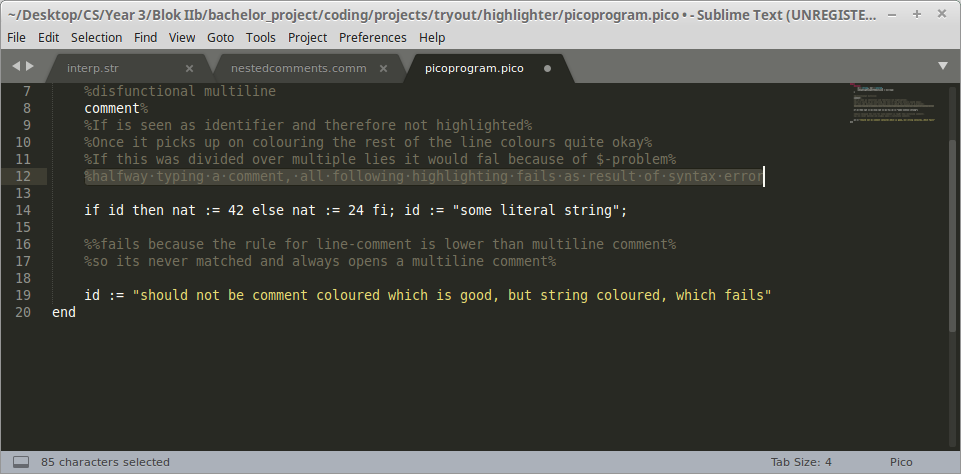
\includegraphics[width=\textwidth, keepaspectratio]{Figures/highlightShots/pico_syntaxError_generated.png}
	\decoRule
 	\caption[Generated highlighter results for Pico grammar with syntax error]{Results of the highlighter on a syntax-error}
 	\label{fig:pico:highlighter:generated:error}
\end{figure}

\pagebreak\subsection{Results of hand-written highlighter}
\begin{figure}[h]
	\centering
	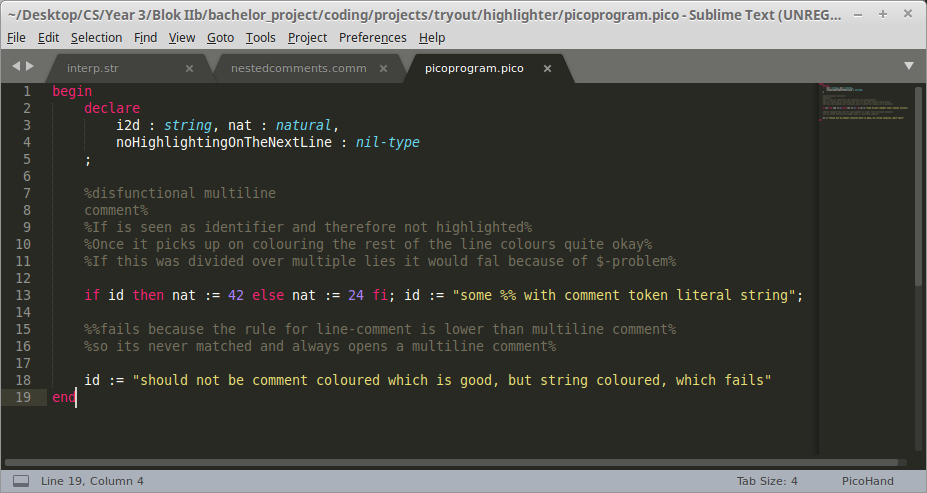
\includegraphics[width=\textwidth, keepaspectratio]{Figures/highlightShots/pico_handwritten.png}
	\decoRule
 	\caption[Hand-written highlighter results for Pico grammar]{Results of the highlighter hand-written for the pico grammar}
 	\label{fig:pico:highlighter:written}
\end{figure}